
The development of concurrent programs is, generally, quite difficult. Several factors can make it even more difficult: for example, it is much harder to write concurrent programs that also need to be correct and efficient (in other words, all of them). Complex programs with many mutexes, or lock-free programs, are harder still.

As was said at the conclusion of the last section, the only hope of managing this complexity is to corral it into small, well-defined sections of the code, or modules. As long as the interfaces and requirements are clear, the clients of these modules don't need to know whether the implementation is lock-free or lock-based. It does affect the performance, so the module may be too slow for a particular need until it's optimized, but we do these optimizations as needed, and they are confined to the particular module.

In this chapter, we focus on the modules that implement data structures for concurrent programming. Why data structures and not algorithms? First of all, there is much more literature on concurrent algorithms out there. Second, most programmers have a much easier time dealing with the algorithms: the code gets profiled, there is a function that takes an excessively long time, we find a different way to implement the algorithm and move on to the next high pole on the performance chart. Then you end up with a program where no single computation takes a large portion of time, but you still have this feeling that it's nowhere as fast as it should be. We have said it before, but it bears repeating: when you have no hot code, you probably have hot data.

The data structures play an even more important role in concurrent programs because they determine what guarantees the algorithms can rely on and what the restrictions are. Which concurrent operations can be done safely on the same data? How consistent is the view of the data as seen by different threads? We cannot write much code if we don't have answers to these questions, and the answers are determined by our choice of the data structures.

At the same time, the design decisions, such as the choice of interfaces and module boundaries, can critically impact the choices we can make when writing concurrent programs. Concurrency cannot be added to a design as an afterthought; the design has to be drawn up with the concurrency in mind from the very beginning, especially the organization of the data.

We begin the exploration of the concurrent data structures by defining a few basic terms and concepts.

\subsubsubsection{6.4.1\hspace{0.2cm}The basics of concurrent data structures}

Concurrent programs that use multiple threads need thread-safe data structures. This seems obvious enough. But what is thread safety, and what makes a data structure thread-safe? At first glance, it seems simple: if a data structure can be used by multiple threads at the same time without any data races (shared between threads), then it is thread-safe.

However, this definition turns out to be too simplistic:

\begin{itemize}
\item It raises the plank very high – for example, none of the STL containers would be considered thread-safe.
\item It carries a very high performance cost.
\item It is often unnecessary, and so is the cost.
\item On top of everything else, it would be completely useless in many cases.
\end{itemize}

Let's tackle these considerations one at a time. Why could a thread-safe data structure be unnecessary even in a multi-threaded program? One trivial possibility is that it is used in a single-threaded portion of the program. We strive to minimize such portions due to their deleterious impact on the overall runtime (remember Amdahl's Law?), but most programs have some, and one of the ways we make such code faster is by not paying unnecessary overhead. The more common scenario for not needing thread safety is when an object is used exclusively by one thread, even in a multi-threaded program. This is very common and very desirable: as we have said several times, shared data is the main source of inefficiency in concurrent programs, so we try to do as much work as possible on each thread independently, using only local objects and data.

But can we be certain that a class or a data structure is safe to use in a multi-threaded program, even if each object is never shared between threads? Not necessarily: just because we do not see any sharing at the interface level does not mean that none is going on at the implementation level. Multiple objects could be sharing the same data internally: static members and memory allocators are just some of the possibilities (we tend to think that all objects that need memory get it by calling malloc() and that malloc() is thread-safe, but a class could implement its own allocator as well).

On the other hand, many data structures are perfectly safe to use in a multi-threaded code as long as none of the threads modify the object. While this may seem obvious, again, we have to consider the implementation: the interface may be read-only, but the implementation may still modify the object. If you think that it is an exotic possibility, consider the standard C++ shared pointer, std::shared\_ptr: when you make a copy of a shared pointer, the copied object is not modified, at least not visibly (it is passed to the constructor of the new pointer by const reference). At the same time, you know that the reference count in the object has to be incremented, which means the copied-from object has changed (shared pointers are thread-safe in this scenario, but this did not happen by accident, and neither is it free, there is a performance cost).

The bottom line is, we need a more nuanced definition of thread safety. Unfortunately, there is no common vocabulary for this very common concept, but there are several popular versions. The highest level of thread safety is often called a strong thread safety guarantee and it means the following: an object that provides this guarantee can be used concurrently by multiple threads without causing data races or other undefined behavior (in particular, any class invariants are preserved). The next level is known as a weak thread safety guarantee. It implies that, first, an object that provides that guarantee can be accessed by multiple threads at once as long as all threads are limited to read-only access (call const member functions of the class), and, second, any thread that has exclusive access to an object can perform any otherwise valid operations on it, no matter what other threads are doing at the same time. An object that does not provide any such guarantee cannot be used in a multi-threaded program at all: even if the object itself is not shared, something inside its implementation is vulnerable to modifications by other threads.

In this book, we will use the language of strong and weak thread-safety guarantees. A class that provides a strong guarantee is sometimes called simply thread-safe. If the class provides only a weak guarantee, it is called thread-compatible. Most STL containers offer this guarantee: if a container is local to one thread, you can use it in any otherwise valid way, but if a container object is shared, you can call only const member functions. Finally, the classes that do not offer any guarantees at all are called thread-hostile and, generally, cannot be used in a multi-threaded program at all.

In practice, we often encounter a mix of strong and weak guarantees: a subset of the interface offers a strong guarantee, but the rest of it provides only the weak guarantee.

So, why do we not try to design every object with a strong thread safety guarantee? The first reason we already mentioned: there is usually performance overhead, the guarantee is often unnecessary because the objects are not shared between threads, and the key to writing an efficient program is not doing any work that can be avoided. The more interesting objection is the one we mentioned earlier, in passing: even in the case where the object is shared in a way that would require thread safety, the strong thread safety guarantee may be useless. Consider this problem: you need to develop a game where the players recruit an army and do battles. The names of all the units in the army are stored in a container, let's say a list of strings. Another container stores the current strength of each unit. During the campaign, the units get killed or recruited all the time, and the gaming engine is multi-threaded and needs to be efficient to manage a large army. While the STL containers provide only the weak thread safety guarantee, let's assume that we have a library of strongly thread-safe containers. It is easy to see that this is not enough: adding a unit requires inserting its name into one container and its initial strength into the other. Both operations are thread-safe by themselves. One thread creates a new unit and inserts it into the first container. Before this thread can also add its strength value, another thread sees the new unit and needs to look up its strength, but there is nothing in the second container yet. The problem is that the thread safety guarantee is offered at the wrong level: from the application point of view, creating a new unit is a transaction, and all gaming engine threads should be able to see the database either before the unit is added or after, but not in the intermediate state. We can accomplish that, for example, by using a mutex: it will be locked before the unit is added and unlocked only after both containers have been updated. However, in this scenario, we don't care about the thread safety guarantees provided by the individual containers, as long as all accesses to these objects are guarded by a mutex anyway. Obviously, what we need instead is a unit database that itself provides the desired thread safety guarantees, for example, by using mutexes. This database may internally use several container objects, and the implementation of the database may or may not need any thread safety guarantees from these containers, but this should be invisible to the clients of the database (having thread-safe containers may make the implementation easier, or not).

This leads us to a very important conclusion: thread safety begins at the design stage. The data structures and the interfaces used by the program must be chosen wisely, so they represent the appropriate level of abstraction and the correct transactions at the level where thread interaction is taking place.

With this in mind, the rest of this chapter should be seen from two sides: on the one hand, we show how to design and implement some basic thread-safe data structures that can be used as building blocks for the more complex (and infinitely more varied) ones you will need in your programs. On the other hand, we also show the basic techniques for building thread-safe classes that can be used to design these more complex data structures.

\subsubsubsection{6.4.2\hspace{0.2cm}Counters and accumulators}

One of the simplest thread-safe objects is a humble counter or its more general form, an accumulator. The counter simply counts some events that can occur on any of the threads. All threads may need to increment the counter or access the current value, so there is potential for a race condition. 

To be of value, we need the strong thread safety guarantee here: the weak guarantee is trivial; reading a value that nobody is changing is always thread-safe. We have already seen the available options for the implementation: a lock of some kind, an atomic operation (when one is available), or a lock-free CAS loop.

The performance of a lock varies with the implementation, but a spinlock is, in general, preferred. The wait time for a thread that did not get immediate access to the counter is going to be very short. So, it does not make sense to incur the cost of putting the thread to sleep and waking it up later. On the other hand, the amount of CPU time wasted because of the busy waiting (polling the spinlock) is going to be negligible, most likely just a few instructions.

The atomic instruction delivers good performance, but the choice of operations is rather limited: in C++, you can atomically add to an integer but not, for example, multiply it. This is enough for a basic counter but may be insufficient for a more general accumulator (the accumulating operation does not have to be limited to a sum). However, if one is available, you just cannot beat the simplicity of an atomic operation.

The CAS loop can be used to implement any accumulator, regardless of the operation we need to use. However, on most modern hardware, it is not the fastest option and is outperformed by a spinlock (see Figure 6.2).

The spinlock can be further optimized for the case when it is used to access a single variable or a single object. Instead of a generic flag, we can make the lock itself be the only reference to the object it is guarding. The atomic variable is going to be a pointer, not an integer, but otherwise, the locking mechanism remains unchanged. The lock() function is non-standard because it returns the pointer to the counter:

\begin{lstlisting}[style=styleCXX]
// 01d_ptrlock_count.C
template <typename T>
class PtrSpinlock {
	public:
	explicit PtrSpinlock(T* p) : p_(p) {}
	T* lock() {
		while (!(saved_p_ =
		p_.exchange(nullptr, std::memory_order_acquire))) {}
	}
	void unlock() {
		p_.store(saved_p_, std::memory_order_release);
	}
	private:
	std::atomic<T*> p_;
	T* saved_p_ = nullptr;
};
\end{lstlisting}

Compared to the earlier implementation of the spinlock, the meaning of the atomic variable is "inverted:" the lock is available if the atomic variable p\_ is not null, otherwise it is taken. All the optimizations we have done for the spinlock are applicable here as well and look exactly the same, so we are not going to repeat them. Also, to be complete, the class needs a set of deleted copy operations (locks are non-copyable). It may be movable if the ability to transfer the lock and the responsibility to release it to another object is desirable. If the lock also owns the object it is pointing to, the destructor should delete it (this combines the functionality of a spinlock and a unique pointer in a single class).

One obvious advantage of the pointer spinlock is that, as long as it provides the only way to access the guarded object, it is not possible to accidentally create a race condition and access the shared data without a lock. The second advantage is that this lock slightly outperforms the regular spinlock more often than not. Whether or not the spinlock also outperforms the atomic operation depends on the hardware as well. The same benchmark yields very different results on different processors:

\hspace*{\fill} \\ %插入空行
\begin{center}
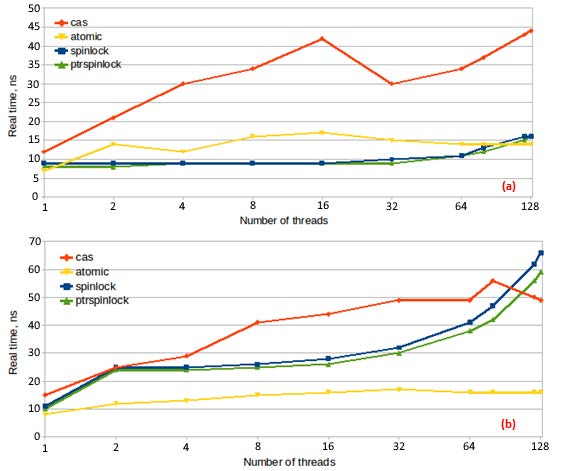
\includegraphics[width=0.9\textwidth]{content/2/chapter6/images/3.jpg}\\
Figure 6.3 – Performance of a shared count increment: regular spinlock, pointer spinlock, lock-free (compare-and-swap, or CAS), and wait-free (atomic) for different hardware systems (a) and (b)
\end{center}

As a rule, the more recent processors handle locks and busy waiting better, and it is more likely that the spinlock delivers better performance on the latest hardware (in Figure 6.3, system b uses Intel X86 CPUs that are one generation behind those in system a).

The average time it takes to execute an operation (or its inverse, the throughput) is the metric that we are mainly concerned with in most HPC systems. However, this is not the only possible metric used to gauge the performance of concurrent programs. For example, if the program runs on a mobile device, the power consumption may be of greater importance. The total CPU time used by all threads is a reasonable proxy for the average power consumption. The same benchmark we used to measure the average real time of the counter increment can be used to measure the CPU time as well:

\hspace*{\fill} \\ %插入空行
\begin{center}
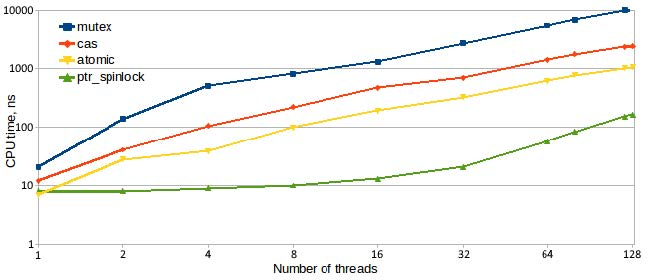
\includegraphics[width=0.9\textwidth]{content/2/chapter6/images/4.jpg}\\
Figure 6.4 – Average CPU time used by different implementations of the thread-safe counter
\end{center}

The bad news here is that no matter the implementation, the cost of accessing the shared data by multiple threads at once increases exponentially with the number of threads, at least when we have many threads (note that the y axis scale in Figure 6.4 is logarithmic). However, the efficiency varies greatly between the implementations, and, at least for the most efficient implementations, the exponential rise does not really kick in until at least eight threads. Note that the results will, again, vary from one hardware system to another, so the choice must be made with your target platform in mind and only after the measurements have been done.

Whatever the chosen implementation, a thread-safe accumulator or a counter should not expose it but encapsulate it in a class. One reason is to provide the clients of the class with a stable interface while retaining the freedom to optimize the implementation.

The second reason is more subtle, and it has to do with the exact guarantees the counter provides. So far, we have focused on the counter value itself, making sure that it is modified and accessed by all threads without any races. Whether or not this is enough depends on how we use the counter. If all we want is to count some events, and nothing else depends on the value of the counter, then we only care that the value itself is correct. On the other hand, if what we are counting is, say, the number of elements in an array, then we are dealing with a data dependency. Let's say that we have a large pre-allocated array (or a container that can grow without disturbing the elements already in it), and all threads are computing new elements to be inserted into this array.  The counter counts the number of elements that are computed and inserted into the array and can be used by other threads. In other words, if a thread reads the value N from the counter, it must be assured that the first N elements of the array are safe to read (which implies that no other thread is modifying them anymore). But the array itself is neither atomic nor protected by a lock. To be sure, we could have protected the access to the entire array by a lock, but this is probably going to kill the performance of the program: if there are many elements already in the array but only one thread can read them at any time, the program might as well be single-threaded. On the other hand, we know that any constant, immutable data is safe to read from multiple threads without any locks. We just need to know where the boundary between the immutable and the changing data is, and that is exactly what the counter is supposed to provide. The key issue here is the memory visibility: we need a guarantee that any changes to the first N elements of the array become visible to all threads before the value of the counter changes from N-1 to N.

We studied memory visibility in the previous chapter when we discussed the memory model. At the time, it might  have appeared to be a largely theoretical matter, but not anymore. From the last chapter, we know that the way we control the visibility is by restricting the memory order or by using memory barriers (two different ways to talk about the same thing). The key difference between a count and an index in a multi-threaded program is that the index provides an additional guarantee: if the thread that increments the index from N-1 to N had completed the initialization of the array element N before it incremented the index, then any other thread that reads the index and gets the value of N (or greater) is guaranteed to see at least N fully initialized and safe to read elements in the array (assuming no other thread writes into these elements, of course). This is a non-trivial guarantee, do not easily dismiss it: multiple threads are accessing the same location in memory (the array element N) without any locking, and one of these threads is writing into this location, and yet, the access is safe, there is no data race. If we could not arrange for this guarantee using the shared index, we would have to lock all accesses to the array, and only one thread would be able to read it at any time. Instead, we can use this atomic index class:

\begin{lstlisting}[style=styleCXX]
// 02_atomic_index.C
class AtomicIndex {
	std::atomic<unsigned long> c_;
	public:
	unsigned long incr() noexcept {
		return 1 + c_.fetch_add(1, std::memory_order_release);
	}
	unsigned long get() const noexcept {
		return c_.load(std::memory_order_acquire);
	}
};
\end{lstlisting}

The only difference between the index at the count is in the memory visibility guarantees; the count offers none:

\begin{lstlisting}[style=styleCXX]
class AtomicCount {
	std::atomic<unsigned long> c_;
	public:
	unsigned long incr() noexcept {
		return 1 + c_.fetch_add(1, std::memory_order_relaxed);
	}
	unsigned long get() const noexcept {
		return c_.load(std::memory_order_relaxed);
	}
};
\end{lstlisting}

The thread safety and memory visibility guarantees should be documented for each of the classes, of course. Whether or not there is a performance difference between the two depends on the hardware. On an X86 CPU, there is none because the hardware instructions for atomic increment and atomic read have the "index-like" memory barriers whether we request them or not. On ARM CPUs, relaxed (or no-barrier) memory operations are noticeably faster. But, regardless of the performance, clarity and intent matter and should not be forgotten: if a programmer uses an index class that explicitly offers the memory order guarantees but does not index anything with it, every reader will wonder what is going on and where is that subtle and hidden place in the code that uses these guarantees. By using the interfaces with the correct set of documented guarantees, you signal to your readers what your intent was when writing this code.

Let us now return to what may be the main "hidden" accomplishment in this section. We learned about thread-safe counters, but along the way, we came up with an algorithm to seemingly violate the first rule of writing multi-threaded code: any time two or more threads access the same memory location and at least one of these threads is writing, all accesses must be locked (or atomic). We did not lock the shared array, we allow arbitrary data in its elements (so it's probably not atomic), and we got away with it! The approach we used to avoid data races turns out to be the cornerstone of almost every data structure designed specifically for concurrency, and we will now take time to better understand and generalize it.

\subsubsubsection{6.4.3\hspace{0.2cm}Publishing protocol}

The general problem we are trying to solve is a very common one in data structure design and, by extension, the development of concurrent programs: one thread is creating new data, and the rest of the program must be able to see this data when it is ready, but not before. The former thread is often called the writer thread or the producer thread. All the other threads are reader or consumer threads.

The most obvious solution is to use a lock and follow the rule of avoiding the data races to the letter. If multiple threads (check) must access the same memory location (check) and at least one thread is writing at this location (exactly one thread in our case – check), then all threads must acquire a lock before accessing this memory location for either reading or writing. The downside of this solution is the performance: long after the producer is done and no more writing happens, all the consumer threads keep locking each other out of reading the data concurrently. Now, read-only access does not require any locking at all, but the problem is, we need to have a guaranteed point in the program such that all the writing happens before this point and all the reading happens after this point. Then we can say that all consumer threads operate in a read-only environment and do not need any locking. The challenge is to guarantee that boundary between reading and writing: remember that, unless we do some sort of synchronization, memory visibility is not guaranteed: just because the writer has finished modifying the memory doesn't mean the reader sees the final state of that memory. The locks include the appropriate memory barriers, as we have seen earlier; they border the critical section and ensure that any operation executed after the critical section will see all the changes to the memory that happened before or during the critical section. But now we want to get the same guarantee without the locks.

The lock-free solution to this problem relies on a very specific protocol for passing information between the producer and the consumer threads:

\begin{itemize}
\item 
The producer thread prepares the data in a memory that is not accessible to other threads. It could be the memory allocated by the producer threads, or it could be pre-allocated memory, but the important point is that the producer is the only thread with a valid reference to this memory, and that valid reference is not shared with other threads (there may be a way for other threads to access this memory, but that would be a bug in the program, similar to indexing an array out of bounds). Since there is only one thread accessing the new data, no synchronization is required. As far as the other threads are concerned, the data simply does not exist.

\item 
All consumer threads must use a single shared pointer for any access to the data, which we call the root pointer, and this pointer is initially null. It remains null while the producer thread is constructing the data. Again, from the point of view of the consumer threads, there is no data at this time. More generally, the "pointer" does not need to be an actual pointer: any kind of handle or reference can be used as long as it gives access to the memory location and can be set to a predetermined invalid value. For example, if all new objects are created in a pre-allocated array, the "pointer" could, in fact, be an index into the array, and the invalid value could be any value greater or equal to the array size.

\item 
The key to the protocol is that the only way for the consumer to access the data is through the root pointer, and this pointer remains null until the producer is ready to reveal, or publish, the data. The act of publishing the data is very simple: the producer must atomically store the correct memory location of the data in the root pointer, and this change must be accompanied by the release memory barrier.

\item 
The consumer thread can, at any time, query the root pointer, again atomically. If the query returns null, then there is no data (as far as the consumer is concerned), and the consumer thread should wait or, ideally, do some other work. If the query returns a non-null value, then the data is ready, and the producer will not change it anymore. The query must be done with the acquire memory barrier, which, in combination with the release barrier on the producer side, guarantees that the new data is visible when the change of the pointer value is observed.
\end{itemize}

This process is sometimes called the publishing protocol because it allows the producer thread to publish information for other threads to consume in a way that guarantees no data races. As we said, the publishing protocol can be implemented using any handle that gives access to the memory as long as this handle can be changed atomically. Pointers are the most common handle, of course, followed by array indices.

The data that is being published can be simple or complex; it doesn't matter. It does not even have to be a single object or a single memory location: the object that the root pointer points to can itself contain pointers to more data. The key elements of the publishing protocol are as follows:

\begin{itemize}
\item
All consumers access a particular set of data through one root pointer. The only way to gain access to the data is to read a non-null value of the root pointer.

\item
The producer can prepare the data any way it wants, but the root pointer remains null: the producer has its own reference to the data that is local to this thread.

\item 
When the producer wants to publish the data, it sets the root pointer to the correct address atomically and with a release barrier. After the data is published, the producer cannot change it (neither can anyone else).

\item 
The consumer threads must read the root pointer atomically and with an acquire barrier. If they read a non-null value, they can read the data accessible through the root pointer.

\end{itemize}

The atomic reads and writes used to implement the publishing protocol should not be, of course, scattered throughout the code. We should implement a publishing pointer class to encapsulate this functionality. In the next section, we will see a simple version of such a class.

\subsubsubsection{6.4.4\hspace{0.2cm}Smart pointers for concurrent programming}

The challenge of concurrent (thread-safe) data structures is how to add, remove, and change the data in a way that maintains certain thread safety guarantees. The publishing protocol, which gives us a way to release new data to all threads, is usually the first step in adding new data to any such data structure. Thus, it should come as no surprise that the first class we will learn about is a pointer that encapsulates this protocol.

\hspace*{\fill} \\ %插入空行
\noindent
\textbf{Publishing pointer}

Here is a basic publishing pointer that also includes the functionality of a unique, or owning, pointer (so we can call it a thread-safe unique pointer):

\begin{lstlisting}[style=styleCXX]
// 03_owning_ptr_mbm.C
template <typename T>
class ts_unique_ptr {
	public:
	ts_unique_ptr() = default;
	explicit ts_unique_ptr(T* p) : p_(p) {}
	ts_unique_ptr(const ts_unique_ptr&) = delete;
	ts_unique_ptr& operator=(const ts_unique_ptr&) = delete;
	~ts_unique_ptr() {
		delete p_.load(std::memory_order_relaxed);
	}
	void publish(T* p) noexcept {
		p_.store(p, std::memory_order_release);
	}
	const T* get() const noexcept {
		return p_.load(std::memory_order_acquire);
	}
	const T& operator*() const noexcept { return *this->get(); }
	ts_unique_ptr& operator=(T* p) noexcept {
		this->publish(p); return *this;
	}
	private:
	std::atomic<T*> p_ { nullptr };
};
\end{lstlisting}

Of course, this is a very bare-bones design; a complete implementation should support a custom deleter, a move constructor and assignment operator, and maybe a few more features, similar to std::unique\_ptr. By the way, the standard does not guarantee that accessing the pointer value stored in a std::unique\_ptr object is atomic or that the necessary memory barriers are used, so the standard unique pointer cannot be used to implement the publishing protocol.

By now, it should be clear to the reader what our thread-safe unique pointer offers: the key functions are publish() and get(), and they implement the publishing protocol. Note that the publish() method does not delete the old data; it is assumed that the producer thread calls publish() only once and only on a null pointer. We could add an assert for that, and it may be a good idea to do so in a debug build, but we are also concerned with the performance. Speaking of performance, a benchmark shows that the single-threaded dereferencing of our publishing pointer takes the same time as that of a raw pointer or of std::unique\_ptr. The benchmark is not complicated:

\begin{lstlisting}[style=styleCXX]
struct A { … arbitrary object for testing … };
ts_unique_ptr<A> p(new A(…));
void BM_ptr_deref(benchmark::State& state) {
	A x;
	for (auto _ : state) {
		benchmark::DoNotOptimize(x = *p);
	}
	state.SetItemsProcessed(state.iterations());
}
BENCHMARK(BM_ptr_deref)->Threads(1)->UseRealTime();
… repeat for desired number of threads …
BENCHMARK_MAIN();
\end{lstlisting}

Running this benchmark gives us an idea of how fast the dereferencing of our lock-free publishing pointer is:

\hspace*{\fill} \\ %插入空行
\begin{center}
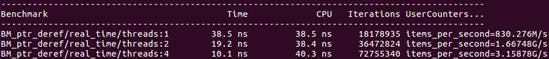
\includegraphics[width=0.9\textwidth]{content/2/chapter6/images/5.jpg}\\
Figure 6.5 – The performance of the publishing pointer (consumer threads)
\end{center}

The result should be compared with dereferencing a raw pointer, which we can also do on multiple threads:

\hspace*{\fill} \\ %插入空行
\begin{center}
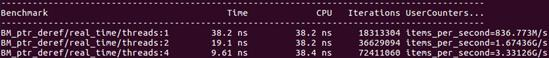
\includegraphics[width=0.9\textwidth]{content/2/chapter6/images/6.jpg}\\
Figure 6.6 – The performance of the raw pointer, for comparison with Figure 6.5
\end{center}

The performance numbers are very close. We can also compare the speed of publishing, but, usually, the consumer side is more important: each object is published only once but then accessed many times.

It is equally important to understand what the publishing pointer does not do. First of all, there is no thread safety in the construction of the pointer. We have assumed that both the producer and the consumer threads share access to the already constructed pointer, which is initialized to null. Who constructed and initialized the pointer? Usually, in any data structure, there is a root pointer through which the entire data structure can be accessed; it was initialized by whatever thread constructed the initial data structure. Then there are pointers that serve as a root for some data element and are themselves contained in another data element. For now, imagine a simple singly linked list where the "next" pointer of every list element is the root for the next element, and the head of the list is the root for the entire list. The thread that produces an element of the list must, among other things, initialize the "next" pointer to null. Then, another producer can add a new element and publish it. Note that this deviates from the general rule that the data, once published, is immutable. This is OK, however, because all changes to the thread-safe unique pointer are atomic. One way or another, it is critical that no thread can access the pointer while it is being constructed (this is a very common restriction, most constructions are not threadsafe, even the question of their thread safety is ill-posed since the object does not exist until it is constructed, so no guarantees can be given).

The next thing our pointer does not do is this: it does not offer any synchronization for multiple producer threads. If two threads attempt to publish their new data elements through the same pointer, the results are undefined, and there is a data race (some consumer threads will see one set of data, and others will see different data). If there is more than one producer thread that operates on a particular data structure, they must use another mechanism for synchronization.

Finally, while our pointer implements a thread-safe publishing protocol, it does nothing to safely "un-publish" and delete the data. It is an owning pointer, so when it is deleted, so is the data it points to. However, any consumer thread can access the data using the value it had acquired earlier, even after the pointer is deleted. The issues of data ownership and lifetime must be handled in some other way. Ideally, we would have a point in the program where the entire data structure or some subset of it is known to be no longer needed; no consumer thread should try to access this data or even retain any pointers to it. At that point, the root pointer and anything accessible through it can be safely deleted. Arranging for such a point in the execution is a different matter entirely; it is often controlled by the overall algorithm.

Sometimes we want a pointer that manages both the creation and the deletion of the data in a thread-safe way. In this case, we need a thread-safe shared pointer.

\hspace*{\fill} \\ %插入空行
\noindent
\textbf{Atomic shared pointer}

If we cannot guarantee that there is a known point in the program where the data can be safely deleted, we have to keep track of how many consumer threads hold valid pointers to the data. If we want to delete this data, we have to wait until there is only one pointer to it in the entire program; then, it is safe to delete the data and the pointer itself (or at least reset it to null). This is a typical job for a shared pointer that does reference counting: it counts how many pointers to the same object are still out there in the program; the data is deleted by the last such pointer.

When talking about thread-safe shared pointers, it is vitally important to understand precisely what guarantees are required from the pointer. The C++ standard shared pointer, std::shared\_ptr, is often referred to as thread-safe. Specifically, it offers the following guarantee: if multiple threads operate on different shared pointers that all point to the same object, then the operations on the reference counter are thread safe even if two threads cause the counter to change at the same time. For example, if one thread is making a copy of its shared pointer while another thread is deleting its shared pointer and the reference count was N before these operations started, the counter will go up to N+1, then back to N (or down first, then up, depending on the actual order of execution) and in the end will have the same value N. The intermediate value could be either N+1 or N-1, but there is no data race, and the behavior is well defined, including the final state. This guarantee implies that the operations on the reference counter are atomic; indeed, the reference counter is an atomic integer and the implementation used fetch\_add() to atomically increment or decrement it.

This guarantee applies as long as no two threads share access to the same shared pointer. How to get each thread its own shared pointer is a separate issue: since all shared pointers pointing to the same object must be created from the very first such pointer, these pointers had to have been passed from one thread to another at some point in time. For simplicity, let us assume, for a moment, that the code that made copies of the shared pointer is protected by a mutex. If two threads access the same shared pointer, then all bets are off. For example, if one thread is trying to copy the shared pointer while another thread is resetting it at the same time, the results are undefined. In particular, the standard shared pointer cannot be used to implement the publishing protocol. However, once the copies of the shared pointer have been distributed to all threads (possibly under lock), the shared ownership is maintained, and the deletion of the object is handled in a thread-safe manner. The object will be deleted once the last shared pointer that points to it is deleted. Note that, since we agreed that each particular shared pointer is never handled by more than one thread, this is completely safe. If, during the execution of the program, the time comes when there is only one shared pointer that owns our object, then there is also only one thread that can access this object. Other threads cannot make copies of this pointer (we don't let two threads share the same pointer object) and don't have any other way to get a pointer to the same object, so the deletion will proceed effectively single-threaded. This is all well and good, but what if we cannot guarantee that two threads won't try to access the same shared pointer? The first example of such access is our publishing protocol: the consumer threads are reading the value of the pointer while the producer thread may be changing it. We need the operations on the shared pointer itself to be atomic. In C++20, we can do just that: it lets us write std::atomic<std::shared\_ptr<T>>. Note that the early proposals featured a new class, std::atomic\_shared\_ptr<T>, instead. In the end, this is not the path that was chosen.

If you do not have a C++20-compliant compiler and the corresponding standard library or cannot use C++20 in your code, you can still do atomic operations on std::shared\_ptr, but you must do so explicitly. In order to publish the object using the pointer p\_ that is shared between all threads, the producer thread must do this:

\begin{lstlisting}[style=styleCXX]
std::shared_ptr<T> p_;
T* data = new T;
… finish initializing the data …
std::atomic_store_explicit(
	&p_, std::shared_ptr<T>(data), std::memory_order_release);
\end{lstlisting}

On the other hand, to acquire the pointer, the consumer thread must do this:

\begin{lstlisting}[style=styleCXX]
std::shared_ptr<T> p_;
const T* data = std::atomic_load_explicit(
	&p_, std::memory_order_acquire).get();
\end{lstlisting}

The major downside of this approach, compared to the C++20 atomic shared pointer, is that there is no protection against accidental non-atomic access. It is up to the programmer to remember to always use atomic functions to operate on the shared pointer.

It should be noted that, while convenient, std::shared\_ptr is not a particularly efficient pointer, and the atomic accesses make it even slower. We can compare the speed of publishing an object using the thread-safe publishing pointer from the last section versus the shared pointer with explicit atomic accesses:

\hspace*{\fill} \\ %插入空行
\begin{center}
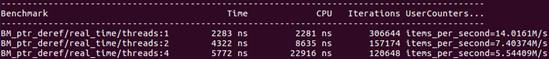
\includegraphics[width=0.9\textwidth]{content/2/chapter6/images/7.jpg}\\
Figure 6.7 – The performance of the atomic shared publishing pointer (consumer threads)
\end{center}

Again, the numbers should be compared with those from Figure 6.5: the publishing pointer is 60 times faster on one thread, and the advantage increases with the number of threads. Of course, the whole point of the shared pointer is that it provides shared resource ownership, so naturally, it takes more time to do more work. The point of the comparison is to show the cost of this shared ownership: if you can avoid it, your program will be much more efficient.

Even if you need shared ownership (and there are some concurrent data structures that are really hard to design without it), usually, you can do much better if you design your own reference-counted pointer with limited functionality and optimal implementation. One very common approach is to use intrusive reference counting. An intrusive shared pointer stores its reference count in the object it points to. When designed for a specific object, such as a list node in our particular data structure, the object is designed with the shared ownership in mind and contains a reference counter. Otherwise, we can use a wrapper class for almost any type and augment it with a reference counter:

\begin{lstlisting}[style=styleCXX]
// 04_intr_shared_ptr_mbm.C
template <typename T> struct Wrapper {
	T object;
	Wrapper(… arguments …) : object(…) {}
	~Wrapper() = default;
	Wrapper (const Wrapper&) = delete;
	Wrapper& operator=(const Wrapper&) = delete;
	std::atomic<size_t> ref_cnt_ = 0;
	void AddRef() {
		ref_cnt_.fetch_add(1, std::memory_order_acq_rel);
	}
	bool DelRef() { return
		ref_cnt_.fetch_sub(1, std::memory_order_acq_rel) == 1;
	}
};
\end{lstlisting}

When decrementing the reference count, it is important to know when it reaches 0 (or was 1 before decrementing): the shared pointer must then delete the object.

The implementation of even the simplest atomic shared pointer is quite lengthy; a very rudimentary example can be found in the sample code for this chapter. Again, this example contains only the bare minimum necessary for the pointer to correctly perform several tasks such as publishing an object and accessing the same pointer concurrently by multiple threads. The aim of the example is to make it easier to understand the essential elements of implementing such pointer (and even then, the code is several pages long).

In addition to using an intrusive reference counter, an application-specific shared pointer can forgo other features of std::shared\_ptr. For example, many applications do not require a weak pointer, but there is an overhead for supporting it even if it's never used. A minimalistic reference-counted pointer can be several times more efficient than the standard one:

%\hspace*{\fill} \\ %插入空行
\begin{center}
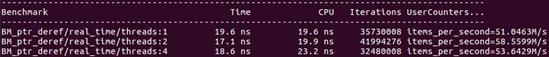
\includegraphics[width=0.9\textwidth]{content/2/chapter6/images/8.jpg}\\
Figure 6.8 – The performance of a custom atomic shared publishing pointer (consumer threads)
\end{center}

It is similarly more efficient for assignment and reassignment of the pointer, atomic exchange of two pointers, and other atomic operations on the pointer. Even this shared pointer is still much less efficient than a unique pointer, so again, if you can manage the data ownership explicitly, without reference-counting, do so.

We now have the two key building blocks of almost any data structure: we can add new data and publish it (reveal it to other threads), and we can track the ownership, even across threads (although it comes at a price).




















